% Intended LaTeX compiler: pdflatex
\documentclass[presentation,t]{beamer}
\usepackage[utf8]{inputenc}
\usepackage[T1]{fontenc}
\usepackage{graphicx}
\usepackage{grffile}
\usepackage{longtable}
\usepackage{wrapfig}
\usepackage{rotating}
\usepackage[normalem]{ulem}
\usepackage{amsmath}
\usepackage{textcomp}
\usepackage{amssymb}
\usepackage{capt-of}
\usepackage{hyperref}
\usepackage{listings}
\usepackage{xcolor}
\usepackage[french, frenchb]{babel}
\usepackage{tikz}
\usetikzlibrary{decorations.pathmorphing, patterns,shapes}
\usetikzlibrary{arrows}
\usetikzlibrary{mindmap,trees}
% Define the layers to draw the diagram
\pgfdeclarelayer{background}
\pgfdeclarelayer{foreground}
\pgfsetlayers{background,main,foreground}
\usepackage{pgfplots}
% \pgfplotsset{compat=1.7}
\pgfplotsset{%
/pgf/number format/.cd,
use comma,
1000 sep={\,},
min exponent for 1000 sep=4
}
\usepackage{mdframed}
\mdfsetup{%
linecolor=gray!40,
linewidth=.7pt,
innertopmargin=0.4em,
innerrightmargin=0.4em,
innerbottommargin=0.4em,
innerleftmargin=0.4em,
leftmargin=1pt,
rightmargin=1pt,
skipabove=4.5pt,
}
\definecolor{mywhite}{HTML}{E3E5E4}
\definecolor{myyellow}{HTML}{EEE039}
\definecolor{myblue}{HTML}{599CEE}
\definecolor{myblack}{HTML}{414141}
\definecolor{myquoteborder}{HTML}{0071C1}
\definecolor{orgmode}{HTML}{048082}
\DeclareUnicodeCharacter{00A0}{~}
\newcommand{\mytitlepage}{%

\includegraphics[height=\paperheight-3cm]{images/org-mode-titlepage}
{\usebeamercolor[fg]{titlegraphic}\inserttitlegraphic\par}
\vfill
\begin{beamercolorbox}[sep=8pt,center]{title}
\usebeamerfont{title}\Huge\inserttitle\par%
\end{beamercolorbox}%
\begin{tikzpicture}[remember picture,overlay,font={\color{orgmode}\Huge\bfseries}]
\node[xshift=0cm,yshift=0cm] at (current page.center) {

\includegraphics[width=\paperwidth]{images/org-mode-titlepage}
};
\node[xshift=-2.7cm,yshift=3.5cm,align=left] at (current page.center) {
Productivité avec \\ l'export \LaTeX
};
\end{tikzpicture}
}
% typeset source code listings
\usepackage{listings}
\usepackage{xcolor}
\definecolor{mc@lstidentifier}{HTML}{000000} % black
\definecolor{mc@lstcomment}{HTML}{008200} % green
\definecolor{mc@lststring}{HTML}{FF5500} % orange
\definecolor{mc@lstkeyword}{HTML}{0000FF} % blue
\definecolor{mc@lstbackground}{HTML}{FFFFCC} % light yellow
\definecolor{mc@lstframe}{HTML}{FFEE88} % dark yellow
\lstdefinelanguage{org}{%
morekeywords={:results, :session, :var, :noweb, :exports},
sensitive=false,
morestring=[b]",
morecomment=[l]{\#},
}
\lstset{%
lineskip=-0.1em,
%
basicstyle=\ttfamily\scriptsize, % font that is used for the code
identifierstyle=\color{mc@lstidentifier},
commentstyle=\color{mc@lstcomment}\itshape,
stringstyle=\color{mc@lststring},
keywordstyle=\color{mc@lstkeyword},
%
extendedchars=true,
inputencoding=utf8,
upquote, %
tabsize=4, % set default tabsize to 4 spaces
showtabs=false, % show tabs within strings adding particular underscores
%  tab=$\to$,
showspaces=false, % show spaces adding particular underscores
showstringspaces=false, % underline spaces within strings
%
numbers=left, % where to put the line numbers
stepnumber=0, % step between two line numbers
numberstyle=\tiny, % line number font size
%
captionpos=b, % set the caption position to `bottom'
%
xleftmargin=0.4em, % text to the right
xrightmargin=0.4em, % text to the left
breaklines=false, % don't break long lines of code
%
frame=single, % add a frame around the code
framexleftmargin=0pt, % frame back to the left
framexrightmargin=0pt, % frame back to the right
backgroundcolor=\color{mc@lstbackground}, % set the background color
rulecolor=\color{mc@lstframe}, % frame color
%
columns=flexible, % try not to ruin the spacing intended by the font designer
keepspaces=true, % don't drop spaces to fix column alignment
%
% mathescape, % allow escaping to (La)TeX mode within $..$
escapechar=², % allow escaping to (La)TeX mode within ²..²
% The backquote was NOT judicious: in some code (comments), I wrap vars
% between such a backquote (`var')
%
% conversion of UTF-8 chars to latin1
literate=
{á}{{\'a}}1
{à}{{\`a}}1
{â}{{\^a}}1
{ä}{{\"a}}1
{ç}{{\c{c}}}1
{é}{{\color{black}\'e}}1
{è}{{\`e}}1
{ê}{{\^e}}1
{ë}{{\"e}}1
{í}{{\'i}}1
{ì}{{\`i}}1
{î}{{\^i}}1
{ï}{{\"i}}1
{ó}{{\'o}}1
{ò}{{\`o}}1
{ô}{{\^o}}1
{ö}{{\"o}}1
{ú}{{\'u}}1
{ù}{{\`u}}1
{û}{{\^u}}1
{ü}{{\"u}}1
{Á}{{\'A}}1
{À}{{\`A}}1
{Â}{{\^A}}1
{Ä}{{\"A}}1
{Ç}{{\c{C}}}1
{É}{{\'E}}1
{È}{{\`E}}1
{Ê}{{\^E}}1
{Ë}{{\"E}}1
{Í}{{\'I}}1
{Ì}{{\`I}}1
{Î}{{\^I}}1
{Ï}{{\"I}}1
{Ó}{{\'O}}1
{Ò}{{\`O}}1
{Ô}{{\^O}}1
{Ö}{{\"O}}1
{Ú}{{\'U}}1
{Ù}{{\`U}}1
{Û}{{\^U}}1
{Ü}{{\"U}}1
}
\definecolor{TeXbackgroundcolor}{HTML}{F1F9EF}
\definecolor{TeXrulecolor}{HTML}{D4E8E3}
\lstdefinestyle{TeX}{backgroundcolor=\color{TeXbackgroundcolor},rulecolor=\color{TeXrulecolor}}
\lstset{breaklines=true}
\usepackage{menukeys}
\let\ORIkeys\keys
\renewcommand{\keys}[1]{\ORIkeys{\texttt{#1}}}
\newcommand{\repeatedkeys}[1]{\keys{\textcolor{gray}{#1}}}
\usetheme{white}
\author{Fabrice Niessen}
\date{\today}
\title{Org-mode LateX export}
\hypersetup{
 pdfauthor={Fabrice Niessen},
 pdftitle={Org-mode LateX export},
 pdfkeywords={org mode, latex, export, babel},
 pdfsubject={Improve your writing productivity with Org mode},
 pdfcreator={Emacs 25.2.1 (Org mode 9.0.8)}, 
 pdflang={Frenchb}}
\begin{document}

\maketitle

\section{Contexte}
\label{sec:org8cf8efc}

\begin{frame}[label={sec:org6694f0c}]{Contexte}
\begin{quote}
Envie d'écrire vos rapports, présentations, examens, thèses et autres
documents aussi facilement qu'un email~?  Besoin de relire~(!) et d'éditer
facilement toutes vos tables et vos listes~?  Besoin d'utiliser des fonctions de
sommation, moyenne ou autre, comme vous le feriez dans un tableur, avec mise à
jour dynamique des résultats~?

Intéressé par l'export conditionnel de parties de vos documents~?  Intéressé par
l'insertion de bouts de code exécutables \emph{in situ} (dans le document)~?  Intéressé
par un export vers de l'HTML, en supplément~?
\end{quote}
\end{frame}

\begin{frame}[label={sec:org763872d}]{Agenda}
\begin{center}
  \begin{tikzpicture}[scale=0.55, transform shape]
    \path[mindmap,concept color=black,text=white,
    level 1 concept/.append style={level distance=130,sibling angle=90}]
      node[concept] {Org}
      [clockwise from=45]
      child[concept color=green!50!black] {
        node[concept] {Syntaxe}
        [clockwise from=105]
        child { node[concept] {Listes} }
        child { node[concept] {Tables} }
        child { node[concept] {Formules} }
      }
      child[concept color=blue] {
        node[concept] {Écrire}
        [clockwise from=75]
        child { node[concept] {Rapports} }
        child { node[concept] {Présentations} }
        child { node[concept] {Examens} }
        child { node[concept] {Thèses} }
        child { node[concept] {Lettres} }
      }
      child[concept color=red] {
        node[concept] {Org Babel}
        [clockwise from=-105]
        child { node[concept] {Coloration} }
        child { node[concept] {Exécution} }
      }
      child[concept color=orange] {
        node[concept] {Export}
        [clockwise from=-135]
        child { node[concept] {LaTeX} }
        child { node[concept] {Beamer} }
        child { node[concept] {HTML} }
        child { node[concept] {ODT} }
      };
  \end{tikzpicture}
\end{center}
\end{frame}

\begin{frame}[label={sec:orgb3221bf}]{Présentation}
\begin{columns}
\begin{column}{.48\columnwidth}
\centering

Org mode

\begin{center}

\includegraphics[width=3cm]{images/org-mode-unicorn.png}
\end{center}
\end{column}

\begin{column}{.48\columnwidth}
\centering

créé en 2003 par \\
Carsten Dominik

\begin{center}
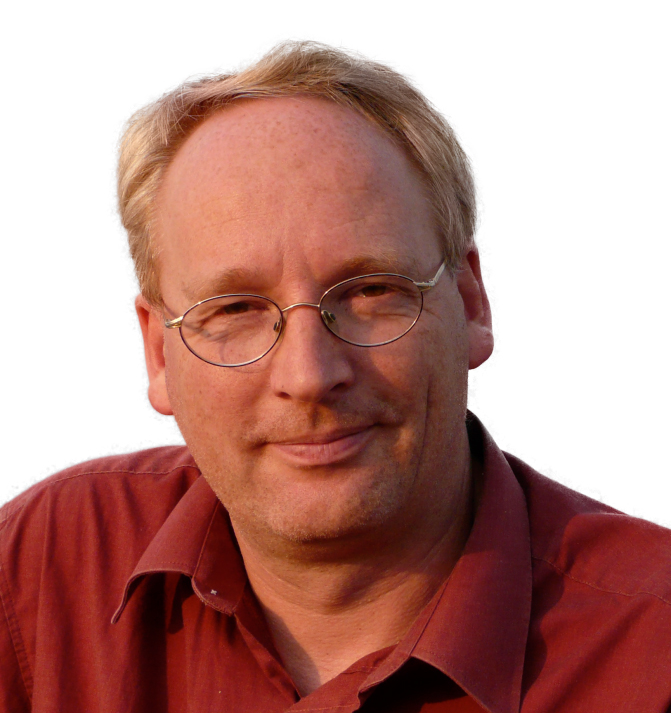
\includegraphics[width=2.6cm]{images/Carsten.png}
\end{center}
\end{column}
\end{columns}

\pause{}

\begin{tikzpicture}[overlay,font={\rmfamily}]
  \node[text width=10.5cm,fill=white,draw=myquoteborder,line width=1pt,inner sep=6pt,rotate=0,xshift=0cm,yshift=-4.1cm] at (current page.center)
  {Back to the future for plain text. (Carsten Dominik)};
\end{tikzpicture}

\pause{}

\begin{tikzpicture}[overlay,font={\rmfamily}]
  \node[text width=10.5cm,draw=myquoteborder,line width=1pt,inner sep=6pt,rotate=0,yshift=-5.2cm] at (current page.center)
  {Org-mode does outlining, note-taking, hyperlinks, spreadsheets, TODO lists,
project planning, GTD, HTML and LaTeX authoring, all with plain text files in
Emacs. (Carsten Dominik)};
\end{tikzpicture}
\end{frame}

\section{Problèmes avec \LaTeX{}}
\label{sec:org2bfb5d3}

\begin{frame}[fragile,label={sec:org350e75e}]{Liste \og à puces\fg{} en \LaTeX{}}
 Code \LaTeX{}

\lstset{language=[LaTeX]TeX,label= ,caption= ,captionpos=b,numbers=none}
\begin{lstlisting}
\begin{itemize}
\item Premier élément
\begin{itemize}
\item Niveau plus profond
\end{itemize}
\item Autre élément
\item Dernier élément
\end{itemize}
\end{lstlisting}

\pause{}

Affichage

\begin{mdframed}
\begin{itemize}
\item Premier élément
\begin{itemize}
\item Niveau plus profond
\end{itemize}
\item Autre élément
\item Dernier élément
\end{itemize}

\end{mdframed}
\end{frame}

\begin{frame}[fragile,label={sec:org1065948}]{Liste numérotée en \LaTeX{}}
 Code \LaTeX{}

\lstset{language=[LaTeX]TeX,label= ,caption= ,captionpos=b,numbers=none}
\begin{lstlisting}
\begin{enumerate}
\item Premier élément
\item Autre élément
\begin{enumerate}
\item Niveau plus profond
\end{enumerate}
\item Dernier élément
\end{enumerate}
\end{lstlisting}

\pause{}

Affichage

\begin{mdframed}
\begin{enumerate}
\item Premier élément
\item Autre élément
\begin{enumerate}
\item Niveau plus profond
\end{enumerate}
\item Dernier élément
\end{enumerate}

\end{mdframed}
\end{frame}

\begin{frame}[fragile,label={sec:org819094f}]{Liste de description en \LaTeX{}}
 Code \LaTeX{}

\lstset{language=[LaTeX]TeX,label= ,caption= ,captionpos=b,numbers=none}
\begin{lstlisting}
\begin{description}
\item[{Premier élément}] Description.
\item[{Autre élément}] Description.
\item[{Dernier élément}] Description.
\end{description}
\end{lstlisting}

\pause{}

Affichage

\begin{mdframed}
\begin{description}
\item[{Premier élément}] Description.
\item[{Autre élément}] Description.
\item[{Dernier élément}] Description.
\end{description}

\end{mdframed}
\end{frame}

\begin{frame}[fragile,label={sec:org2d7399d}]{Tableau en \LaTeX{}}
 \begin{columns}
\begin{column}{0.48\columnwidth}
Code \LaTeX{}

\lstset{language=[LaTeX]TeX,label= ,caption= ,captionpos=b,numbers=none}
\begin{lstlisting}
\begin{table}[!htbp]
\caption{\label{tab:org306b011}
Tableau avec alignement}
\centering
\begin{tabular}{lr}
Mois & Montant\\
\hline
Janvier & 1565\\
Fevrier & 1164\\
Mars & 740\\
Avril & 2273\\
Mai & 1688\\
Juin & 2942\\
\end{tabular}
\end{table}
\end{lstlisting}

\pause{}
\end{column}

\begin{column}{0.48\columnwidth}
Affichage

\begin{mdframed}
\begin{table}[!htbp]
\caption{\label{achats-par-mois}Tableau avec alignement}
\centering
\begin{tabular}{lr}
Mois & Montant\\
\hline
Janvier & 1565\\
Fevrier & 1164\\
Mars & 740\\
Avril & 2273\\
Mai & 1688\\
Juin & 2942\\
\end{tabular}
\end{table}

\end{mdframed}
\end{column}
\end{columns}
\end{frame}

\begin{frame}[fragile,label={sec:org6de4c34}]{Tableau en \LaTeX{}}
 \begin{itemize}
\item Pour \emph{Open Office Calc}
\begin{enumerate}
\item Installer la macro \emph{Calc2LaTeX}
\item Utiliser cette macro
\begin{enumerate}
\item Construire le tableau avec le tableur
\item Sélectionner la partie intéressante du tableau
\item Lancer la macro de conversion en code \LaTeX{}
\item Enregistrer le résultat dans un fichier \texttt{<fichier>.tex}
\item Insérer \texttt{\textbackslash{}input\{<fichier>\}} là où le tableau doit apparaître
\end{enumerate}
\end{enumerate}

\item Pour \emph{Excel} \\
Installer et utiliser la macro \emph{Excel2LaTeX}
\end{itemize}

\pause{}

\begin{center}
  \begin{tikzpicture}[font={\rmfamily}]
    \node[text width=5.7cm,draw=myquoteborder,line width=1pt,inner sep=6pt,rotate=-5]
    {Fichier LaTeX et fichier du tableur à garder synchronisés... \\ Manuellement... \\ À chaque édition...};
  \end{tikzpicture}
\end{center}
\end{frame}

\begin{frame}[plain,label={sec:orgbbfd3f0}]{Mais on a toujours fait comme cela\ldots{}}
\setbeamertemplate{navigation symbols}{}
\begin{tikzpicture}[remember picture,overlay]
    \node[xshift=0cm,yshift=0cm] at (current page.center) {
        
\includegraphics[width=\paperwidth]{images/stop}
    };
\end{tikzpicture}

\begin{tikzpicture}[remember picture,overlay,font={\Large\bfseries\color{white}}]
  \node[xshift=3.2cm,yshift=0cm,align=center] at (current page.center)
    {Il est \\ temps de changer \\ d'outils !};
\end{tikzpicture}
\end{frame}

\section{Solutions avec Org}
\label{sec:org5d0ecd8}

\begin{frame}[plain,label={sec:orge888991}]{Org à la rescousse}
\setbeamertemplate{navigation symbols}{}
\begin{tikzpicture}[remember picture,overlay]
    \node[xshift=0cm,yshift=0cm] at (current page.center) {
        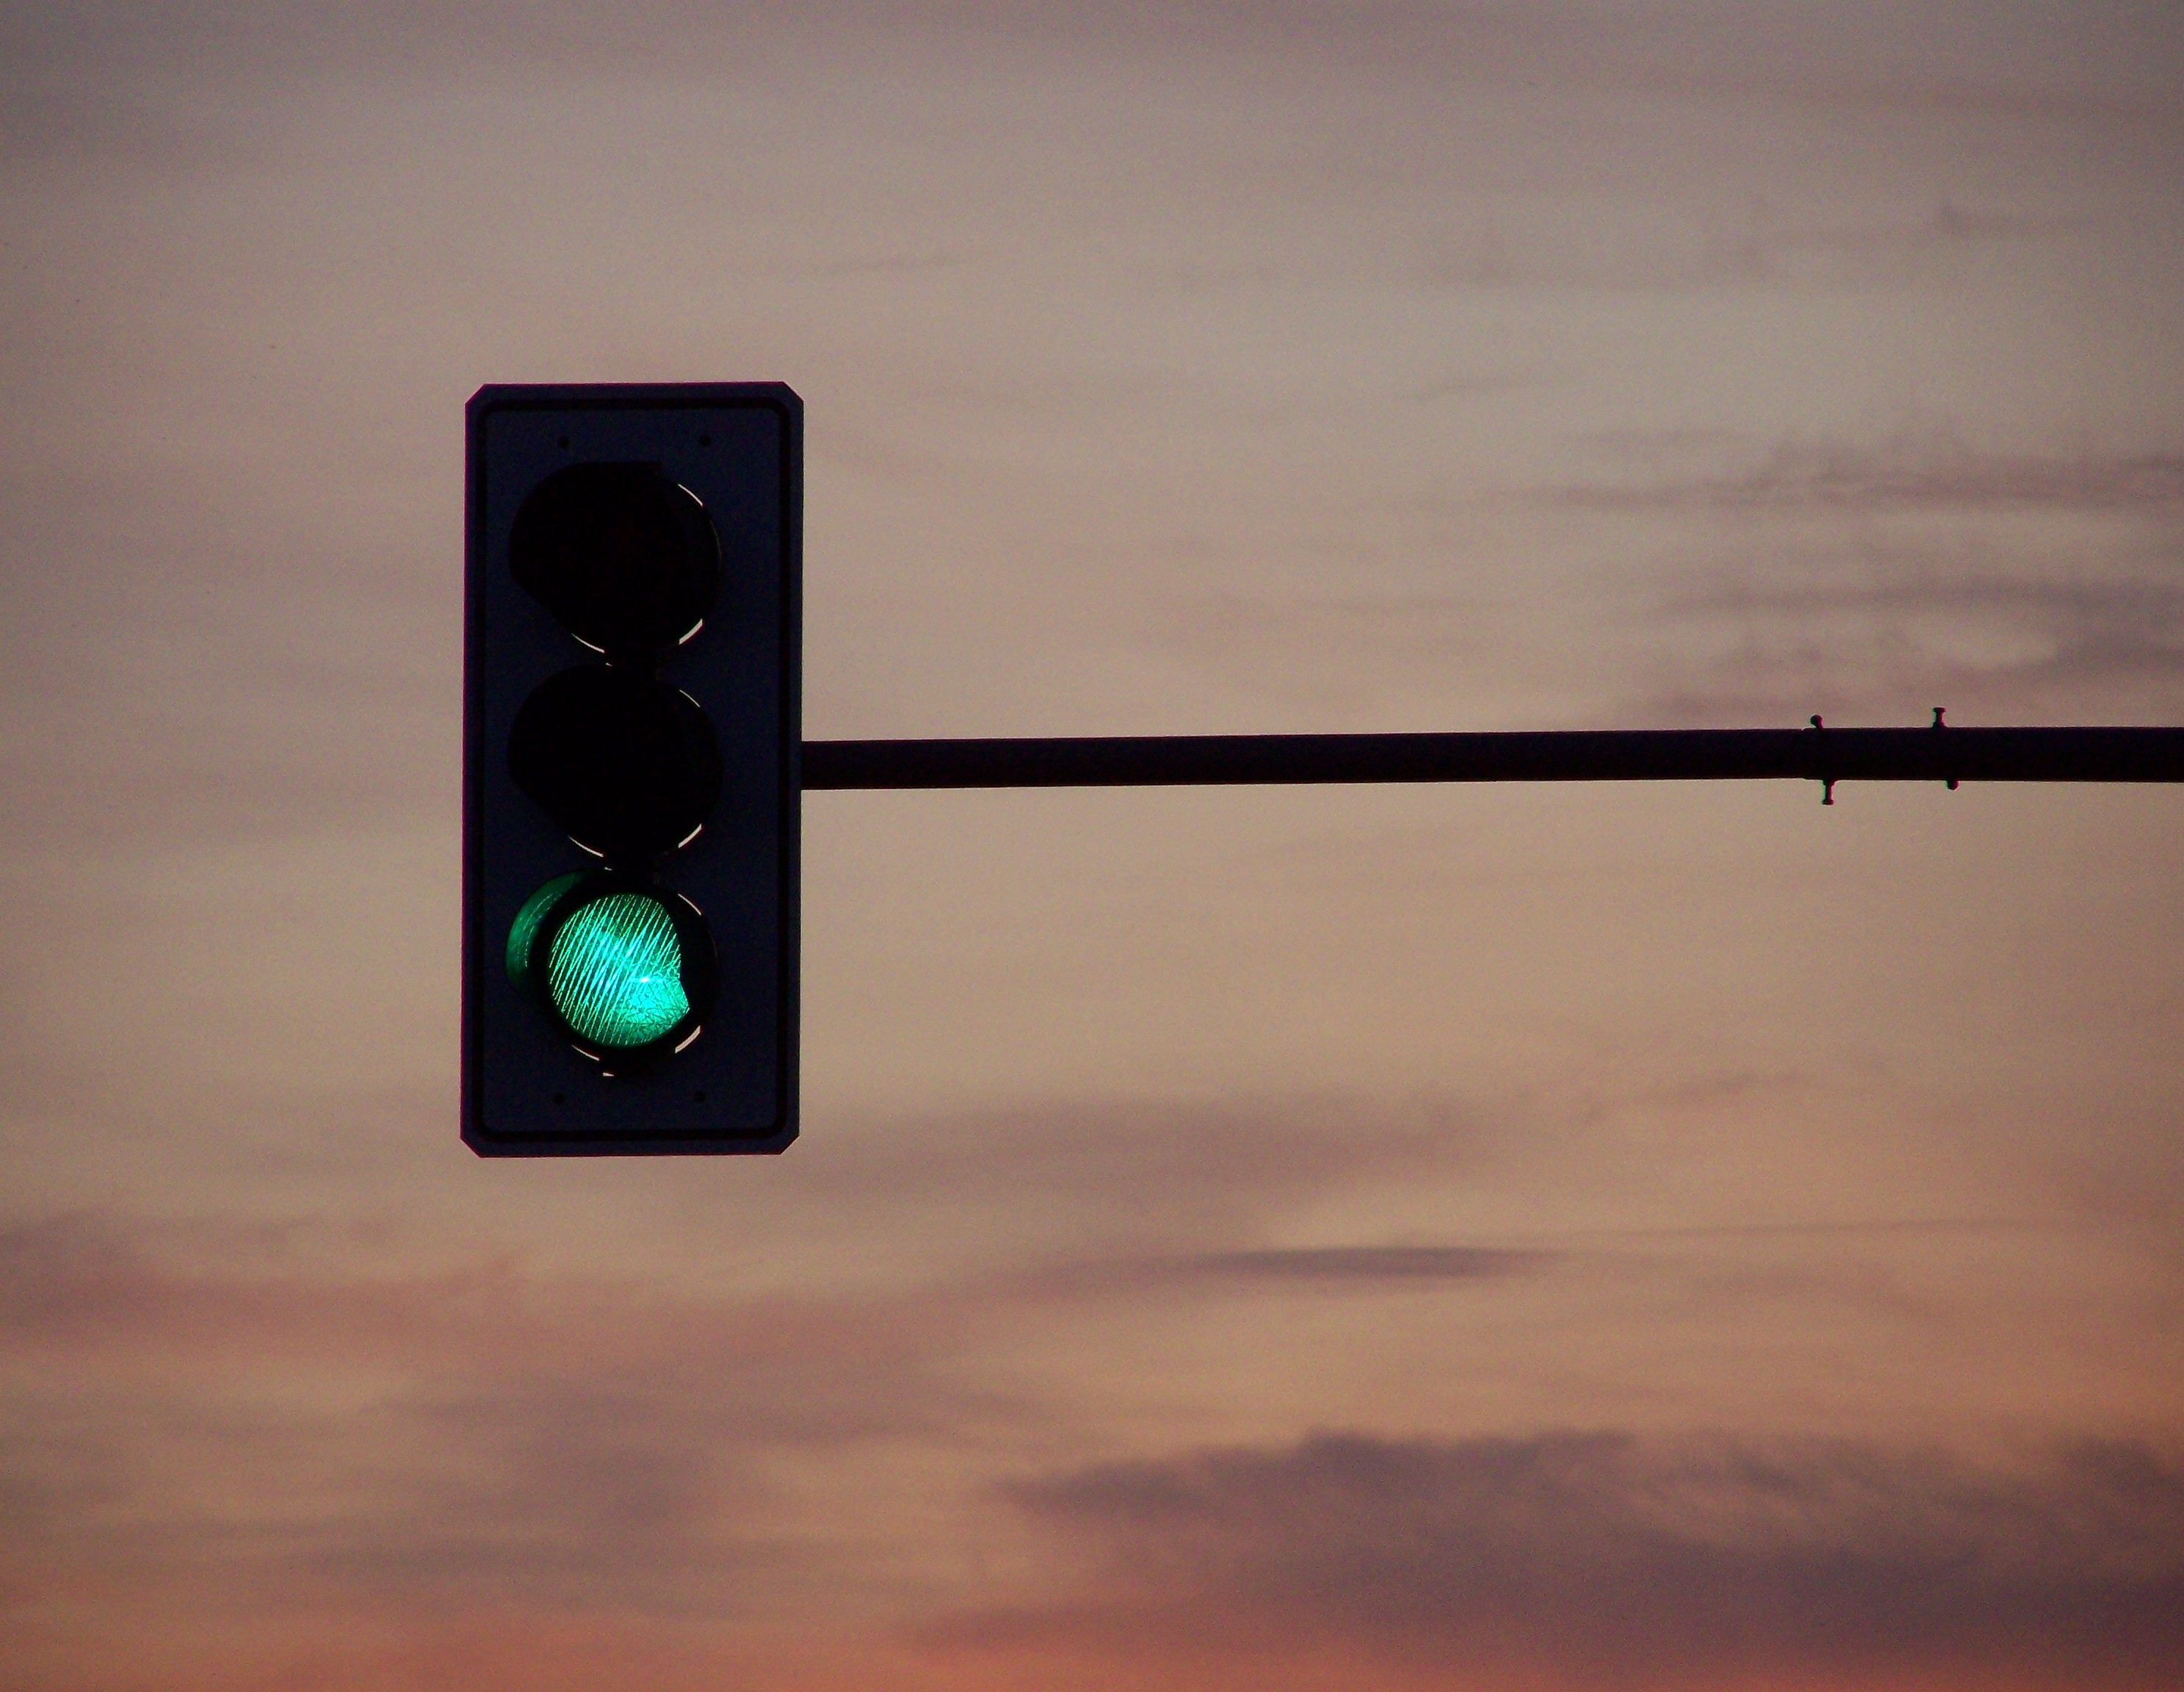
\includegraphics[width=\paperwidth]{images/green-stop-light}
    };
\end{tikzpicture}

\begin{tikzpicture}[remember picture,overlay]
  \node[xshift=2cm,yshift=-0.8cm] at (current page.center)
    {\Large\bfseries{}
    \color{myblack}En route avec \color{mywhite}Org mode};
\end{tikzpicture}
\end{frame}

\begin{frame}[fragile,label={sec:org210635c}]{Mise en forme}
 Balisage virtuellement inexistant

\begin{columns}
\begin{column}{0.48\columnwidth}
\lstset{language=org,label=org890dace,caption= ,captionpos=b,numbers=none}
\begin{lstlisting}
Normal

*Gras*

/Italique/

_Souligné_

=Code=

~Verbatim~
\end{lstlisting}
\end{column}

\begin{column}{0.48\columnwidth}
\begin{mdframed}
Normal

\textbf{Gras}

\emph{Italique}

\uline{Souligné}

\texttt{Code}

\verb~Verbatim~

\end{mdframed}

\pause{}
\end{column}
\end{columns}

Marqueurs cachés dans le \emph{buffer} Org avec

\lstset{language=[LaTeX]TeX,label= ,caption= ,captionpos=b,numbers=none}
\begin{lstlisting}
(setq org-hide-emphasis-markers t)      ; dans votre .emacs
\end{lstlisting}
\end{frame}

\begin{frame}[fragile,label={sec:orgfe3fb38}]{Liste \og à puces\fg{} en Org mode}
 Affichage

\begin{mdframed}
\begin{itemize}
\item Premier élément
\begin{itemize}
\item Niveau plus profond
\end{itemize}
\item Autre élément
\item Dernier élément
\end{itemize}

\end{mdframed}

\pause{}

Syntaxe Org

\lstset{language=org,label= ,caption= ,captionpos=b,numbers=none}
\begin{lstlisting}
- Premier élément
  - Niveau plus profond
- Autre élément
- Dernier élément
\end{lstlisting}

\pause{}

Assistance à l'édition~: espaces devant les tirets pour chaque \emph{item} des sous-listes
\end{frame}

\begin{frame}[fragile,label={sec:org885cccc}]{Liste numérotée en Org mode}
 Affichage

\begin{mdframed}
\begin{enumerate}
\item Premier élément
\item Autre élément
\begin{enumerate}
\item Niveau plus profond
\end{enumerate}
\item Dernier élément
\end{enumerate}

\end{mdframed}

\pause{}

Syntaxe Org

\lstset{language=org,label= ,caption= ,captionpos=b,numbers=none}
\begin{lstlisting}
1. Premier élément
2. Autre élément
   1. Niveau plus profond
3. Dernier élément
\end{lstlisting}

\pause{}

Assistance à l'édition~: numéros pour chaque \emph{item} des (sous-) listes numérotées
\end{frame}

\begin{frame}[fragile,label={sec:org9e04a95}]{Liste de description en Org mode}
 Affichage

\begin{mdframed}
\begin{description}
\item[{Premier élément}] Description.
\item[{Autre élément}] Description.
\item[{Dernier élément}] Description.
\end{description}

\end{mdframed}

\pause{}

Syntaxe Org

\lstset{language=org,label= ,caption= ,captionpos=b,numbers=none}
\begin{lstlisting}
- Premier élément :: Description.
- Autre élément :: Description.
- Dernier élément :: Description.
\end{lstlisting}
\end{frame}

\begin{frame}[fragile,label={sec:org9ebe203}]{Tableau en Org mode}
 \begin{columns}
\begin{column}{0.42\columnwidth}
Affichage

\begin{mdframed}
\begin{table}[!htbp]
\caption{\label{achats-par-mois}Tableau avec alignement}
\centering
\begin{tabular}{lr}
Mois & Montant\\
\hline
Janvier & 1565\\
Fevrier & 1164\\
Mars & 740\\
Avril & 2273\\
Mai & 1688\\
Juin & 2942\\
\end{tabular}
\end{table}

\end{mdframed}

\pause{}
\end{column}

\begin{column}{0.55\columnwidth}
Syntaxe Org

\lstset{language=org,label= ,caption= ,captionpos=b,numbers=none}
\begin{lstlisting}
#+CAPTION: Tableau avec alignement
#+ATTR_LaTeX: :align lr
#+name: achats-par-mois
| Mois    | Montant |
|---------+---------|
| Janvier |    1565 |
| Fevrier |    1164 |
| Mars    |     740 |
| Avril   |    2273 |
| Mai     |    1688 |
| Juin    |    2942 |
\end{lstlisting}

où les tirets =  filet horizontal

(Utiliser \texttt{:align |l|r|} \\
pour les filets verticaux)

\pause{}
\end{column}
\end{columns}

\alert{Limitation} --- \\
Fusion de cellules (actuellement) impossible dans des tables Org
\end{frame}

\begin{frame}[label={sec:org4c2afcb}]{Création de tableaux}
\begin{itemize}
\item À partir de rien
\begin{itemize}
\item Insérer 2 barres verticales
\item Appuyer sur \keys{TAB}
\item Pour insérer une nouvelle ligne, appuyer sur \keys{M-S-down}
\item Pour insérer une nouvelle colonne, appuyer sur \keys{M-S-right}
\end{itemize}

\item À partir de données formatées en colonne, appuyer sur \keys{C-c |}
\begin{itemize}
\item Données séparées par \keys{TAB}
\item Données séparées par une virgule (CSV)
\item Données séparées par un ou plusieurs espaces consécutifs
\end{itemize}
\end{itemize}
\end{frame}

\begin{frame}[label={sec:orgd03260c}]{Édition de tableaux}
\begin{itemize}
\item Pour supprimer
\begin{itemize}
\item \keys{M-S-up} --- la ligne courante
\item \keys{M-S-left} --- la colonne courante
\end{itemize}
\item Pour déplacer la ligne courante
\begin{itemize}
\item \keys{M-up} --- vers le haut
\item \keys{M-down} --- vers le bas
\end{itemize}
\item Pour déplacer la colonne courante
\begin{itemize}
\item \keys{M-left} --- vers la gauche
\item \keys{M-right} --- vers la droite
\end{itemize}
\item Numériques alignés à droite par défaut
\end{itemize}
\end{frame}

\begin{frame}[label={sec:org79a42ff}]{Édition de tableaux}
\begin{itemize}
\item \keys{S-RET} --- Copier le contenu de la cellule supérieure ou courante (en
fonction du contexte)
\item \keys{C-c C-c} --- Réaligner la table
\item \keys{C-c -} --- Insérer une ligne horizontale
\end{itemize}
\end{frame}

\begin{frame}[fragile,label={sec:org0cad686}]{Tableur}
 \begin{itemize}
\item Référence absolue (format interne) \texttt{@L\$C}

\lstset{language=org,label= ,caption= ,captionpos=b,numbers=none}
\begin{lstlisting}
     $1   $2
@1 |    |    |
@2 |    |    |
\end{lstlisting}

\item Référence relative \texttt{@+L\$-C}
\begin{itemize}
\item Omettre la ligne ou colonne, si ligne ou colonne \alert{courante}
\end{itemize}

\item Référence symbolique
\begin{itemize}
\item \keys{@<} ou \texttt{\$<} --- Première ligne ou colonne
\item \keys{@<<} ou \texttt{\$<<} --- Deuxième ligne ou colonne
\item \ldots{}
\item \keys{@>>} ou \texttt{\$>>} --- Avant-dernière ligne ou colonne
\item \keys{@>} ou \texttt{\$>} --- Dernière ligne ou colonne
\end{itemize}
\end{itemize}
\end{frame}

\begin{frame}[fragile,label={sec:org444932a}]{Références}
 \begin{itemize}
\item Ligne horizontale
\begin{itemize}
\item \keys{@I} --- Première \emph{hline}
\item \keys{@II} --- Deuxième \emph{hline}
\item \ldots{}
\item \keys{@-I} --- Première \emph{hline} au-dessus de la ligne courante
\item \keys{@+I} --- Première \emph{hline} en-dessous de la ligne courante
\end{itemize}

\item \emph{Range} \texttt{@L\$C..@L\$C}

\item Référence externe \keys{remote(nom-de-table,référence)}
\end{itemize}
\end{frame}

\begin{frame}[fragile,label={sec:org0704cb8}]{Formules}
 \begin{columns}
\begin{column}{0.55\columnwidth}
Syntaxe Org

\lstset{language=org,label=orgb795f32,caption= ,captionpos=b,numbers=none}
\begin{lstlisting}
#+CAPTION: Tableau avec formule
#+ATTR_LaTeX: :align lr
#+name: achats-par-mois
| Mois    | Montant |
|---------+---------|
| Janvier |    1565 |
| Fevrier |    1164 |
| Mars    |     740 |
| Avril   |    2273 |
| Mai     |    1688 |
| Juin    |    2942 |
|---------+---------|
| Total   |   10372 |
#+TBLFM: @>$2=vsum(@-I..@-II)
\end{lstlisting}
\end{column}

\begin{column}{0.42\columnwidth}
Affichage

\begin{mdframed}
\begin{table}[!htbp]
\caption{\label{achats-par-mois}Tableau avec formule}
\centering
\begin{tabular}{lr}
Mois & Montant\\
\hline
Janvier & 1565\\
Fevrier & 1164\\
Mars & 740\\
Avril & 2273\\
Mai & 1688\\
Juin & 2942\\
\hline
Total & 10372\\
\end{tabular}
\end{table}

\end{mdframed}
\end{column}
\end{columns}
\end{frame}

\begin{frame}[fragile,label={sec:orge85cac4}]{Formules}
 \begin{itemize}
\item Insérer une formule
\begin{itemize}
\item \keys{C-c =} --- Insérer une formule \alert{colonne} \texttt{\$C=}
\item \keys{C-u C-c =} --- Insérer une formule \alert{cellule} \texttt{@L\$C=}
\item À la main --- Insérer une formule \alert{range de cellules en ligne} \texttt{@L\$C..@L\$C=}
\end{itemize}

\item Recalculer
\begin{itemize}
\item \keys{C-c *} --- Ré-appliquer les formules\ldots{} pour la \alert{ligne courante}
\item \keys{C-u C-c *} --- \ldots{} pour toutes les lignes de la table
\item \keys{C-u C-u C-c *} --- \ldots{} jusqu'à ce que la \alert{table} soit \alert{stable}
\end{itemize}
\end{itemize}
\end{frame}

\begin{frame}[label={sec:org8627e29}]{Fonctions}
\begin{itemize}
\item Voir manuel de GNU Emacs Calc

\item Math
\begin{center}
\begin{tabular}{ll}
\keys{vsum(range)} & Somme\\
\keys{vprod(range)} & Produit\\
\keys{exp(x)} & Exponentielle\\
\keys{sin(x)} & Sinus\\
\keys{cos(x)} & Cosinus\\
\keys{tan(x)} & Tangente\\
\end{tabular}
\end{center}
\end{itemize}
\end{frame}

\begin{frame}[label={sec:org279200a}]{Fonctions}
\begin{itemize}
\item Statistique
\begin{center}
\begin{tabular}{ll}
\keys{vmean(range)} & Moyenne arithmétique\\
\keys{vmedian(range)} & Médiane\\
\keys{vmin(range)} & Minimum\\
\keys{vmax(range)} & Maximum\\
\keys{vcount(range)} & Nombre de valeurs\\
\keys{vgmean(range)} & Moyenne géométrique\\
\keys{vsdev(range)} & Déviation standard \og sample\fg{}\\
\keys{vpdev(range)} & Déviation standard \og population\fg{}\\
\keys{vvar(range)} & Variance\\
\end{tabular}
\end{center}

\item Logique
\begin{center}
\begin{tabular}{ll}
\keys{if(test,val-true,val-false)} & Condition\\
\end{tabular}
\end{center}

\item Texte
\begin{center}
\begin{tabular}{ll}
\keys{string("")} & \emph{String} vide\\
\end{tabular}
\end{center}
\end{itemize}
\end{frame}

\begin{frame}[fragile,label={sec:orgeed629d}]{Format}
 \begin{center}
\begin{tabular}{ll}
\texttt{\%.nf} & \emph{Float} avec \emph{n} décimales pour \texttt{printf}\\
\keys{t} & Durée (sous forme de fraction)\\
\keys{T} & Durée (sous forme \texttt{HH:MM:SS})\\
\end{tabular}
\end{center}
\end{frame}

\begin{frame}[fragile,label={sec:orgf92099b}]{Assistance à l'édition de la ligne \texttt{\#+TBLFM}}
 \begin{itemize}
\item \texttt{C-c \}} --- Inverser l'affichage des références
\item \keys{C-u C-u C-c =} --- Éditer une formule dans le tableau
\begin{itemize}
\item \keys{C-c ?} --- Mettre en évidence les cellules référencées au point
\end{itemize}
\item \keys{C-c '} --- Éditer les formules dans un \emph{buffer} spécial
\begin{itemize}
\item \keys{S-up/down/left/right} --- Modifier la référence courante
\end{itemize}
\item \texttt{C-c \{} --- Activer le débogueur (montrer l'historique de substitution pour les
formules)
\end{itemize}
\end{frame}

\begin{frame}[fragile,label={sec:org0bdaf97}]{Tableau Org dans source \LaTeX{}}
 \begin{itemize}
\item Utiliser un environnement \texttt{comment}

\lstset{language=[LaTeX]TeX,label= ,caption= ,captionpos=b,numbers=none}
\begin{lstlisting}
% BEGIN RECEIVE ORGTBL montantdesachats
% END RECEIVE ORGTBL montantdesachats
\begin{comment}
#+ORGTBL: SEND montantdesachats orgtbl-to-latex
| Mois    | HTVA | TVAC |
|---------+------+------|
| Janvier | 1565 | 1887 |
| Février | 1164 | 1404 |
| Mars    |  740 |  892 |
|---------+------+------|
| Total   | 3469 | 4183 |
#+TBLFM: $3=$2*1.206;%.0f::@>$2..@>$3=vsum(@2..@4)
% $ (optional extra dollar to keep font-lock happy)
\end{comment}
\end{lstlisting}

\item Appuyer sur \keys{C-c C-c} pour exporter le tableau en \LaTeX{}
\end{itemize}
\end{frame}

\begin{frame}[fragile,label={sec:org75c3732}]{Code en R}
 \alert{Générer un diagramme en bâtons}, où teinte = taille relative

Syntaxe Org

\lstset{language=org,label= ,caption= ,captionpos=b,numbers=none}
\begin{lstlisting}
#+name: exemple-R-plot-function
#+headers: :var data=achats-par-mois
#+headers: :exports results
#+begin_src R :results graphics :file images/Rplots.png
rel.hts <- (data$Montant / max(data$Montant)) / 2
grays <- gray(1 - rel.hts)

barplot(data$Montant,
        col = grays,
        main = "Achats par mois",
        names.arg = data$Mois,
        ylab = "Montant (EUR)")
#+end_src
\end{lstlisting}
\end{frame}

\begin{frame}[label={sec:orgbf41703}]{Graphique généré en R}
\begin{columns}
\begin{column}{0.36\columnwidth}
\begin{table}[!htbp]
\caption{\label{tab:orgf8d7735}
Achats par mois}
\centering
\begin{tabular}{lr}
Mois & Montant\\
\hline
Janvier & 1565\\
Fevrier & 1164\\
Mars & 740\\
Avril & 2273\\
Mai & 1688\\
Juin & 2942\\
\end{tabular}
\end{table}

\begin{tikzpicture}[remember picture,overlay,font={\rmfamily}]
  \node<4->[text width=4cm,draw=myquoteborder,line width=1pt,inner sep=6pt,
            xshift=-3.7cm,yshift=-3.2cm,rotate=5] at (current page.center)
  {Données source, code et résultat dans le même document Org};
\end{tikzpicture}

\pause{}

\begin{tikzpicture}[remember picture,overlay]
  \tikzset{
      myarrow/.style={->, >=latex', shorten >=1pt},
  }
  % This is drawn in the foreground
  \begin{pgfonlayer}{foreground}
    \node[circle,fill=yellow,xshift=-2.1cm,yshift=3cm] (c) at (current page.center) {Code R};
    \draw[thick] (c.west) -- ++(-.7,0) -- ++(0,-.7);
    \draw<3->[thick,myarrow] (c.east) -- ++(.7,0) -- ++(0,-.7);
  \end{pgfonlayer}
\end{tikzpicture}

\pause{}
\end{column}

\begin{column}{0.60\columnwidth}
\begin{center}
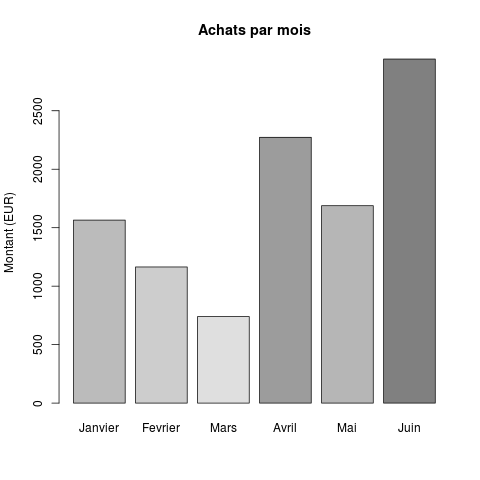
\includegraphics[height=7.5cm]{images/Rplots.png}
\end{center}

\pause{}
\end{column}
\end{columns}
\end{frame}

\begin{frame}[label={sec:org443ad94}]{Graphique généré en PGFPlots}
\begin{columns}
\begin{column}{0.36\columnwidth}
\begin{tikzpicture}[font={\rmfamily}]
  \node[text width=4cm,draw=myquoteborder,line width=1pt,inner sep=6pt,rotate=0]
  {Même table source};
\end{tikzpicture}

\begin{tikzpicture}[font={\rmfamily}]
  \node<2->[text width=4cm,draw=myquoteborder,line width=1pt,inner sep=6pt,rotate=0]
  {Autre code};
\end{tikzpicture}

\begin{tikzpicture}[font={\rmfamily}]
  \node<3->[text width=4cm,draw=myquoteborder,line width=1pt,inner sep=6pt,rotate=0]
  {Nouveau résultat};
\end{tikzpicture}
\end{column}

\begin{column}{0.60\columnwidth}
\pgfplotsset{width=7cm}
\begin{onlyenv}<1-3>
  \begin{tikzpicture}
   \begin{axis}[ymin=0,title={Achats par mois}, ymin=0, ylabel={Montant (EUR)}, ybar,
                symbolic x coords={Janvier,Fevrier,Mars,Avril,Mai,Juin},
                x tick label style={rotate=45, anchor=north east, inner sep=0mm}]
     \addplot+[
     scatter,
     only marks,
     colormap={test}{
       color=(blue!10); color=(blue!70)
     },
     scatter/use mapped color={draw=blue,fill=mapped color},
     scatter/@pre marker code/.append code={
         \pgfkeys{/pgf/fpu=true,/pgf/fpu/output format=fixed}
         \pgfmathsetmacro\negheight{-\pgfplotspointmeta}
         \fill [draw=blue] (-10.5pt,10.5pt) rectangle
         ([xshift=10.5pt]axis direction cs:Janvier,\negheight);
         \pgfplotsset{mark=none}
       },
     ]
      plot coordinates {
        (Janvier,1565)
        (Fevrier,1164)
        (Mars,740)
        (Avril,2273)
        (Mai,1688)
        (Juin,2942)
      };
    \end{axis}
  \end{tikzpicture}
\end{onlyenv}
\end{column}
\end{columns}
\end{frame}

\begin{frame}[fragile,label={sec:org626b07e}]{Code SQL}
 \lstset{language=org,label= ,caption= ,captionpos=b,numbers=none}
\begin{lstlisting}
#+PROPERTY:  header-args :eval never :engine msosql :cmdline -S 192.168.31.46 -U user -P secret -d ARCHIBUS -n -w 700 :results value :exports both :noweb yes
\end{lstlisting}

\lstset{language=SQL,label= ,caption= ,captionpos=b,numbers=none}
\begin{lstlisting}
SELECT ctry_id, city_id
FROM bl
ORDER BY ctry_id
\end{lstlisting}

\begin{center}
\begin{tabular}{ll}
ctry\_id & city\_id\\
\hline
AT & Vienna\\
BE & Brussels\\
DE & Berlin\\
DE & Munich\\
NL & The Hague\\
\end{tabular}
\end{center}
\end{frame}

\begin{frame}[fragile,label={sec:org7b07040}]{Autres environnements}
 Blocs spéciaux

\lstset{language=org,label= ,caption= ,captionpos=b,numbers=none}
\begin{lstlisting}
#+BEGIN_EXPORT latex
#+END_EXPORT
\end{lstlisting}

\lstset{language=org,label= ,caption= ,captionpos=b,numbers=none}
\begin{lstlisting}
#+begin_note
#+end_note
\end{lstlisting}
\end{frame}

\begin{frame}[fragile,label={sec:org5ab1a9a}]{Sectionnement}
 Une étoile par niveau de profondeur

\lstset{language=org,label= ,caption= ,captionpos=b,numbers=none}
\begin{lstlisting}
  * Heading de niveau 1
  ** Heading de niveau 2
  *** Heading de niveau 3
  **** Heading de niveau 4
  ...
\end{lstlisting}

Insérer un nouvel \emph{heading} avec \keys{M-RET}
\end{frame}

\begin{frame}[label={sec:org5644433}]{Édition de la structure}
\begin{itemize}
\item \alert{Section}
\begin{itemize}
\item \keys{M-left} --- Promouvoir la section
\item \keys{M-right} --- \og Démouvoir\fg{} la section
\end{itemize}

\item \alert{Sous-arbre}
\begin{itemize}
\item \keys{M(-S)-up} --- Déplacer le sous-arbre vers le haut
\item \keys{M(-S)-down} --- Déplacer le sous-arbre vers le bas
\item \keys{M-S-left} --- Promouvoir le sous-arbre
\item \keys{M-S-right} --- \og Démouvoir\fg{} le sous-arbre
\end{itemize}
\end{itemize}
\end{frame}

\begin{frame}[fragile,label={sec:orgdad56a0}]{Visibilité}
 \lstset{language=org,label= ,caption= ,captionpos=b,numbers=none}
\begin{lstlisting}
* Introduction...
* Expériences...
* Résultats...
* Conclusions...
\end{lstlisting}

\begin{itemize}
\item \keys{S-TAB} --- Cycler, dans tout le \alert{fichier}, entre 3 états
\begin{enumerate}
\item Afficher les niveaux 1 uniquement
\item Afficher tous les niveaux
\item Afficher tout
\end{enumerate}

\item \keys{TAB} --- Cycler, dans un \alert{sous-arbre}, entre 3 états
\begin{enumerate}
\item Afficher le niveau courant uniquement
\item Afficher les niveaux enfants directs
\item Afficher tout
\end{enumerate}
\end{itemize}
\end{frame}

\begin{frame}[fragile,label={sec:org171f4db}]{Écrire un rapport}
 \lstset{language=org,label= ,caption= ,captionpos=b,numbers=none}
\begin{lstlisting}
#+TITLE:     Productivité avec l'export LaTeX d'Org mode
#+AUTHOR:    Fabrice Niessen
#+EMAIL:     (concat "fniessen" at-sign "pirilampo.org")
#+DESCRIPTION: Subject
#+KEYWORDS:  org mode, export, latex
#+LANGUAGE:  fr
#+OPTIONS:   H:2
\end{lstlisting}

\begin{itemize}
\item Insérer un \emph{template} avec les options (par défaut) d'export via \keys{C-c C-e #}

\item \emph{Smart quotes} : guillemets à la française si
\begin{itemize}
\item \emph{Babel} est chargé
\item Langue définie = \texttt{fr}
\end{itemize}

\item Mettre l'option \keys{H:2}
\begin{itemize}
\item (Sous-)sections numérotées jusqu'au niveau 2
\item Niveaux suivants non-numérotés
\end{itemize}

\item À vous d'écrire le reste\ldots{}
\end{itemize}
\end{frame}

\begin{frame}[fragile,label={sec:org136c094}]{Générer un index}
 \begin{itemize}
\item Écrire des entrées d'index

\lstset{language=org,label= ,caption= ,captionpos=b,numbers=none}
\begin{lstlisting}
#+index: Org-mode
#+index: Definitions!Org-mode
\end{lstlisting}

\item Placer l'index à l'endroit désiré

\item Produire l'index en mettant à jour \texttt{org-latex-pdf-process}

\lstset{language=org,label= ,caption= ,captionpos=b,numbers=none}
\begin{lstlisting}
#+BIND: org-latex-pdf-process ("pdflatex %b" "bibtex %b" "pdflatex %b" "pdflatex %b")
\end{lstlisting}
\end{itemize}
\end{frame}

\begin{frame}[fragile,label={sec:org926617a}]{Écrire une présentation}
 \begin{itemize}
\item Charger \texttt{ox-beamer}

\item Insérer un \emph{template} d'options pour l'export avec \\
\texttt{M-x org-beamer-insert-options-template}

\lstset{language=org,label= ,caption= ,captionpos=b,numbers=none}
\begin{lstlisting}
#+LaTeX_CLASS: beamer
#+LaTeX_CLASS_OPTIONS: [presentation]
#+BEAMER_THEME: mc
#+COLUMNS: %45ITEM %10BEAMER_env(Env) %10BEAMER_act(Act) %4BEAMER_col(Col) %8BEAMER_opt(Opt)
#+PROPERTY: BEAMER_col_ALL 0.1 0.2 0.3 0.4 0.5 0.6 0.7 0.8 0.9 0.0 :ETC
\end{lstlisting}

\item Utiliser le mode mineur \texttt{org-beamer-mode} pour ajouter certaines propriétés

\item Mettre l'option \keys{H:2}
\begin{itemize}
\item Sections en niveau 1
\item \emph{Frames} en niveau 2
\end{itemize}
\end{itemize}
\end{frame}

\begin{frame}[fragile,label={sec:orgae5b150}]{Écrire un examen}
 Export des questions avec ou sans les solutions.

\lstset{language=org,label= ,caption= ,captionpos=b,numbers=none}
\begin{lstlisting}
#+OPTIONS: d:(not "SOLUTION")

:QUESTION:
#+begin_src emacs-lisp
(+ 1 1)
#+end_src
:END:

:SOLUTION:
#+begin_src emacs-lisp
2
#+end_src
:END:
\end{lstlisting}

où \texttt{d:t} donnerait l'\emph{output} entier.

D'autres solutions sont possibles (avec \texttt{EXCLUDE\_TAGS}, par exemple).
\end{frame}

\begin{frame}[label={sec:orgbb426dd}]{Écrire une documentation logicielle}
La \og \href{http://fr.wikipedia.org/wiki/Programmation\_lettrée}{programmation littéraire}\fg{} (\alert{literate programming}, Knuth) = écrire la
documentation sur le code source (dans l'ordre requis par la logique) en même temps
et \emph{en un même lieu} que le code

\pause{}

\begin{description}
\item[{Tangle}] Extraire les blocs de code source et générer le code \og emmêlé\fg{}, formaté
pour la machine (pour compilation ou exécution ultérieure)
\end{description}

\begin{center}
  \begin{tikzpicture}[font={\rmfamily}]
    \node[text width=8.5cm,draw=myquoteborder,line width=1pt,inner sep=6pt,rotate=5]
    {Possibilité de changer l'ordre du code source, via l'argument Noweb};
  \end{tikzpicture}
\end{center}

\pause{}

\begin{description}
\item[{Weave}] Exporter le fichier Org en entier comme documentation \og tissée\fg{}, formatée
pour l'homme (généralement en \LaTeX{} ou en HTML)
\end{description}
\end{frame}

\begin{frame}[fragile,label={sec:orgc9fa9e4}]{Coloration syntaxique}
 \begin{itemize}
\item À l'export

\lstset{language=java,label= ,caption= ,captionpos=b,numbers=none}
\begin{lstlisting}
  /* affiche simplement la chaîne "Hello World!" sur la
   * sortie standard */
  class HelloWorldApp {
      public static void main(String[] args) {
          System.out.println("Hello World!");
      }
  }
\end{lstlisting}

\item \alert{Dans le \emph{buffer} Org} lui-même (équivalent de \emph{multiple major modes})
\end{itemize}
\end{frame}

\begin{frame}[label={sec:orgc069716}]{Écrire une thèse}
Exécution des blocs de code \emph{in situ} (dans le document)

\begin{itemize}
\item En usage \alert{interactif} (\keys{C-c C-v C-e})
\item Pendant l'opération de \alert{tangle} (\keys{C-c C-v C-t})
\item Pendant l'\alert{export} \LaTeX{}, HTML, ou autre (\keys{C-c C-e}) --- sans besoin de \emph{Makefile}
\end{itemize}

\pause{}

Cela vous permet d'insérer, \emph{dans votre document}, toutes les \alert{données} (qui
peuvent être raisonnablement incluses) et blocs de \alert{code} que vous avez
utilisés, suivant ainsi les principes de la \alert{recherche reproductible}

\begin{tikzpicture}[remember picture,overlay,font={\rmfamily}]
  \draw<3->node[text width=2.8cm,draw=myquoteborder,line width=1pt,inner sep=6pt,
        rotate=5,xshift=-2.4cm,yshift=-2.2cm] at (current page.center)
  {Référentiel des connaissances};
  \draw<4->node[text width=2.3cm,draw=myquoteborder,line width=1pt,inner sep=6pt,
        fill=white,rotate=-5,xshift=0.8cm,yshift=-2.7cm] at (current page.center)
  {Compendium};
\end{tikzpicture}
\end{frame}

\begin{frame}[fragile,label={sec:org241e236}]{Exécution de blocs de code}
 \begin{itemize}
\item Appeler \texttt{org-babel-do-load-languages}

\lstset{language=Lisp,label= ,caption= ,captionpos=b,numbers=none}
\begin{lstlisting}
(org-babel-do-load-languages
 'org-babel-load-languages
 '((R . t)
   (awk . t)
   (calc . t)
   (dot . t)
   (emacs-lisp . t)
   (gnuplot . t)
   (latex . t)
   (org . t)
   (python . t)
   (shell . t)
   (sql . t)))
\end{lstlisting}

pour éviter \emph{No org-babel-execute function for xxx!}

\item On peut enchaîner les blocs de code, même dans des langages différents

\item Usages
\begin{itemize}
\item Insérer le contenu d'une table dans une BD SQL
\end{itemize}
\end{itemize}
\end{frame}

\begin{frame}[fragile,label={sec:org06ba580}]{Mathématiques}
 Syntaxe \LaTeX{} pour les équations

\lstset{language=[LaTeX]TeX,label= ,caption= ,captionpos=b,numbers=none}
\begin{lstlisting}
\[
\left( \int_{0}^{\infty} \frac{\sin x}{\sqrt x}\,\mathrm{d}x \right)^{2} -
\prod_{k=1}^{\infty} \frac{4k^{2}}{4k^{2}-1} +
\frac{\lambda}{2n}\sum_{k=1} ^{n} \theta_{k} ^{2} x^{n} = 0
\]
\end{lstlisting}

\[
\left( \int_{0}^{\infty} \frac{\sin x}{\sqrt x}\,\mathrm{d}x \right)^{2} -
\prod_{k=1}^{\infty} \frac{4k^{2}}{4k^{2}-1} +
\frac{\lambda}{2n}\sum_{k=1} ^{n} \theta_{k} ^{2} x^{n} = 0
\]
\end{frame}

\begin{frame}[fragile,label={sec:org86db6b6}]{Écrire une lettre}
 \keys{M-x load-library RET ox-koma-letter RET}

\keys{C-c C-e k o} ou \\
\keys{C-c C-e C-s k o} (\keys{C-s} pour sélectionner le sous-arbre courant)

\lstset{language=org,label= ,caption= ,captionpos=b,numbers=none}
\begin{lstlisting}
* Une lettre par section
:PROPERTIES:
:EXPORT_LATEX_CLASS: malettre
:EXPORT_LCO: DefaultAddress
:EXPORT_AUTHOR: Fabrice Niessen
:EXPORT_DATE: 12 juin 2013
:EXPORT_TO_ADDRESS: Denis Bitouzé \\
:EXPORT_TO_ADDRESS: 220 avenue de l'Université \\
:EXPORT_TO_ADDRESS: 59379 Dunkerque
:EXPORT_OPENING: Cher Monsieur,
:EXPORT_CLOSING: Sincèrement,
:EXPORT_OPTIONS: backaddress:nil
:END:

Lorem ipsum dolor sit amet, consectetur adipisicing elit, sed do eiusmod
tempor incididunt ut labore et dolore magna aliqua.

**                                                        :PS:

Ut enim ad minim veniam.
\end{lstlisting}
\end{frame}

\begin{frame}[label={sec:orgea4761d}]{Exporter le document Org}
\begin{tikzpicture}[remember picture]
  \tikzset{product/.style={rotate=10,fill=blue,opacity=.10,text opacity=1},
           link/.style={->,>=latex,thick}}
  \node (org) at (0,0) {
\includegraphics[width=2.8cm]{images/org-mode-unicorn}};
  \node (exporters) at (6,0) {
\includegraphics[width=4cm]{images/icon-all-formats}};
  \draw<1->[link] (org) -- (exporters);
  \node at (2.6,0.2) {C-c C-e};
  \draw<1->node[product] at (exporters) {Dispatcher};
  \draw<2->node (pdf) at (3.5,-4) {
\includegraphics[width=2.5cm]{images/icon-pdf}};
  \draw<2->[link] (exporters) -- (pdf);
%  \draw<2->node at (0,2.2) {l};
  \draw<2->node[product] at (pdf) {LaTeX + Beamer};
  \draw<3->node (html) at (6.3,-4) {
\includegraphics[width=2.5cm]{images/icon-html}};
  \draw<3->[link] (exporters) -- (html);
%  \draw<3->node at (-0.5,3) {h};
  \draw<4->node[align=left] (rest) at (9,-4) {- Texte \\ - \textbf{ODT} \\ - Man \\ - \textbf{Markdown} \\ - Texinfo \\ - etc.};
  \draw<4->[link] (exporters) -- (rest);
\end{tikzpicture}%

\begin{tikzpicture}[overlay,font={\rmfamily}]
  \draw<5->node[text width=3.5cm,fill=white,draw=myquoteborder,line width=1pt,inner sep=6pt,rotate=-10,xshift=4.5cm,yshift=0.9cm] at (current page.center)
  {Répéter la dernière commande d'export avec C-u C-c C-e};
\end{tikzpicture}
\end{frame}

\begin{frame}[label={sec:org5cca4a6}]{Exporter en Beamer}
\begin{columns}
\begin{column}{0.48\columnwidth}
\begin{center}
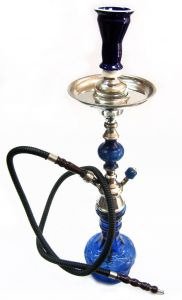
\includegraphics[width=90px]{images/narghile.jpg}
\end{center}
\end{column}

\begin{column}{0.48\columnwidth}
{\fontfamily{frc}\selectfont\Large%
Ceci n'est pas une pipe
}

\pause{}
\end{column}
\end{columns}

{\centering

Mais \href{https://github.com/fniessen/stage-latex-dunkerque-2013/blob/master/org-mode-latex-export.org}{ceci} est une présentation Beamer \\
composée en Org mode \\
exportée avec \keys{C-c C-e l P}

(après avoir fait \keys{M-x load-library RET ox-beamer RET})

}
\end{frame}

\begin{frame}[fragile,label={sec:org4d8f9be}]{Exports à jour}
 \lstset{language=Lisp,label= ,caption= ,captionpos=b,numbers=none}
\begin{lstlisting}
  (with-eval-after-load "org"

    (defun org-save-buffer-and-do-related ()
      "Save buffer, execute/tangle code blocks, and export to HTML/PDF."
      (interactive)
      (let* ((orgfile (buffer-file-name))
             (base-name (file-name-base orgfile))
             (htmlfile (concat base-name ".html"))
             (pdffile (concat base-name ".pdf")))
        (save-buffer)
        (when (derived-mode-p 'org-mode)
          (org-babel-execute-buffer)
          (let ((before-save-hook nil))
            (save-buffer))
          (org-babel-tangle)
          (when (file-exists-p htmlfile)
            (if (file-newer-than-file-p orgfile htmlfile)
                (org-html-export-to-html)
              (message "HTML is up to date with Org file")))
          (when (file-exists-p pdffile)
            (if (file-newer-than-file-p orgfile pdffile)
                (if (string-match "^#\\+BEAMER_THEME: " (buffer-string))
                    (org-beamer-export-to-pdf)
                  (org-latex-export-to-pdf))
              (message "PDF is up to date with Org file")))
          (beep))))

    (define-key org-mode-map
      (kbd "<f9>") 'org-save-buffer-and-do-related))
\end{lstlisting}
\end{frame}

\begin{frame}[label={sec:org5788ab2}]{Suppléments non abordés}
\begin{itemize}
\item Statut \keys{TODO} / \keys{DONE} sur les sections
\item \emph{Tags} \keys{:noexport:} sur les sections
\item Agenda
\item Pointeuse du temps de travail
\item Recherche avancée (multi-fichiers)
\item etc.
\end{itemize}
\end{frame}

\section{Conclusion}
\label{sec:orgc0519dd}

\begin{frame}[<+->][label={sec:orgf41dd6e}]{Cliquer ici}
Pour en apprendre plus sur Org mode

\begin{itemize}
\item Manuels de référence
\begin{itemize}
\item \href{http://orgmode.org/orgcard.pdf}{Org mode Reference Card} (2 pages)
\item \href{http://orgmode.org/orgguide.pdf}{The compact Org mode Guide} (\textpm{} 40 pages)
\item \href{http://orgmode.org/org.pdf}{The Org Manual} (\textpm{} 250 pages)
\end{itemize}

\item \href{http://orgmode.org/worg/org-faq.html}{FAQ Org mode}

\item Site \href{http://orgmode.org/worg/}{Worg} (= \og Wiki\fg{} sur Org mode)

\item Liste de discussion \href{mailto:emacs-orgmode@gnu.org}{emacs-orgmode@gnu.org}
\end{itemize}

\begin{tikzpicture}[remember picture,overlay,font={\rmfamily}]
  \draw<6->node[text width=3.5cm,draw=myquoteborder,line width=1pt,inner sep=6pt,rotate=-5,xshift=4.2cm,yshift=0.3cm] at (current page.center)
  {Écrit en Org \\ Publié en HTML};
\end{tikzpicture}
\end{frame}

\begin{frame}[label={sec:org9e42837}]{Conclusion}
\begin{itemize}
\item \LaTeX{} reste l'outil de tout premier plan pour créer des documents écrits de
grande qualité

\item Mais on gagne sur plusieurs terrains, et on l'étend dans plein de
directions, en l'utilisant en tant que \emph{backend} d'Org mode

\item Rédiger un document ou une présentation devient aussi simple que d'écrire un
\emph{email}
\end{itemize}
\end{frame}

\begin{frame}[plain,label={sec:org45182a2}]{Conclusion}
\setbeamertemplate{navigation symbols}{}
\begin{tikzpicture}[remember picture,overlay]
    \node[xshift=0cm,yshift=0cm] at (current page.center) {
        
\includegraphics[height=\paperheight]{images/homme-fort}
    };
\end{tikzpicture}

\begin{tikzpicture}[remember picture,overlay,font={\large\fontsize{12}{22}\bfseries}]
  \node[xshift=-3.3cm,yshift=3.0cm,align=left] at (current page.center)
    {\color{mywhite}Soyez \color{myyellow}PLUS EFFICACE \\
     \color{mywhite}et \color{myyellow}PLUS PRODUCTIF\color{mywhite} \\
     \color{mywhite}avec Org mode !};
  \node[xshift=-3.8cm,align=left] at (current page.center)
    {\color{mywhite}Téléchargez \color{myyellow}Org 9 \\ \color{mywhite}dès aujourd'hui};
  \node[xshift=-3.5cm,yshift=-1.2cm,align=left] at (current page.center)
    {\tiny\color{myyellow}git clone git://orgmode.org/org-mode.git};
  \node[xshift=-4.7cm,yshift=-1.5cm,align=left] at (current page.center)
    {\tiny\color{myyellow}make autoloads};
  \node[xshift=-2.8cm,yshift=-1.8cm,align=left] at (current page.center)
    {\tiny\color{myyellow}(add-to-list 'load-path "<path-to-repo>/lisp/") ; <- adjust};
  \node[xshift=5.5cm,yshift=-2.3cm,align=left] at (current page.center)
    {\color{myyellow}Merci};
\end{tikzpicture}
\end{frame}

\begin{frame}[label={sec:org952d4a8}]{Coordonnées}
Fabrice Niessen \\
(concat \og fniessen\fg{} at-sign \og \href{http://www.pirilampo.org/}{pirilampo.org}\fg{})

Consultant IT @ \href{http://www.pirilampo.be/}{Pirilampo SPRL} \\
Auteur @ \href{http://www.pirilampo.org/}{Pirilampo.org}

\begin{columns}
\begin{column}{0.48\columnwidth}
\href{https://github.com/fniessen}{GitHub} fniessen \\
\href{http://be.linkedin.com/pub/fabrice-niessen/0/a42/200}{LinkedIn} fabrice-niessen \\
\href{http://www.slideshare.net/fniessen}{SlideShare} fniessen \\
\href{https://twitter.com/f\_niessen}{Twitter} f\_niessen \\
\end{column}

\begin{column}{0.48\columnwidth}
Vous avez des idées~? \\
Contactez-moi~!
\end{column}
\end{columns}
\end{frame}
\end{document}
